\documentclass[11pt, oneside]{article} 
\usepackage{geometry}
\geometry{letterpaper} 
\usepackage{graphicx}
	
\usepackage{amssymb}
\usepackage{amsmath}
\usepackage{parskip}
\usepackage{color}
\usepackage{hyperref}

\graphicspath{{/Users/telliott/Github/figures/}}
% \begin{center} \includegraphics [scale=0.4] {gauss3.png} \end{center}

\title{Sum of angles}
\date{}

\begin{document}
\maketitle
\Large

%[my-super-duper-separator]

\label{sec:sum_angles_similar_tri}

\subsection*{cosine of a sum}

The sum of angle formulas (for the sine and cosine of the sum or difference of two angles) are used often in calculus, not only for solving problems, but even in finding an expression for the derivative of sine and cosine.

You really must know them.  I think it's so important that we will show several ways of finding these formulas.  The proofs are also beautiful, which helps to explain why I've included so many.

The easiest way to remember them uses Euler's equation.  We'll see that toward the end.

There are four equations, one each for $\sin s \pm t$ and $\cos s \pm t$.

I've memorized only one:
\[ \cos s - t = \cos s \cos t + \sin s \sin t \]

By $\cos s - t$ we mean $\cos (s - t)$, but have left off the parentheses.  Say "cos cos" and then recall the difference in sign, minus on the left, plus on the right.

\subsection*{check with $s = t$}

I like this version because it can be checked easily.  Just set $s = t$:
\[ \cos s - t = \cos s - s = \cos 0 = 1 = \cos^2 s + \sin^2 s \]
which is our favorite trigonometric identity and obviously correct.

\subsection*{derivation 0}
I'm calling this one derivation zero because it was added later, and it is really a simplified form of derivation 1.  We draw two triangles, one on top of the other, with the hypotenuse of the second scaled to be equal to $1$.  Then draw a rectangle around the whole thing.

\begin{center} \includegraphics [scale=0.4] {sum_angles_6.png} \end{center}

For the triangle with angle $\theta$ and hypotenuse $1$, the labels should be obvious.

Second, for triangles with angle $\phi$ where the hypotenuse is \emph{not} $1$, we have something like $\cos \phi \cos \theta$ on the bottom of the figure, which gives the desired value $\cos \phi$ after dividing by the hypotenuse, $\cos \theta$.

The angle labeled $\theta + \phi$ at the top is known by the alternate interior angles theorem.

Now, just read off the relationships from the sides of the rectangle:
\[ \sin \phi + \theta = \sin \phi \cos \theta + \cos \phi \sin \theta \]
\[ \cos \phi + \theta = \cos \phi \cos \theta - \sin \phi \sin \theta \]

And what's really nice is that a simple change will give the difference formulas:

\begin{center} \includegraphics [scale=0.4] {sum_angles_7.png} \end{center}
We've changed the symbol $\phi$ to refer to the complementary angle from what it was before.  

We can justify the label $\phi - \theta$ for the angle at the lower left in various ways, for example, by adding up the three angles at that corner:
\[ (\phi - \theta) + \theta + (90 - \phi) = 90 \]

Switch the labels appropriately (it's easy since this $\phi$ is the complement of the old one).

Read the result:
\[ \sin \phi - \theta = \sin \phi \cos \theta - \cos \phi \sin \theta \]
\[ \cos \phi - \theta = \cos \phi \cos \theta + \sin \phi \sin \theta \]

\subsection*{derivation 1}

Here is a geometric derivation of the sum of angles formulas for both sine and cosine.  The key is to draw an inspired diagram.

Construct a right triangle, with one of the smaller angles labeled $s$.  Then construct another right triangle with small angle $t$, with the hypotenuse of the first triangle containing angle $s$ as the base adjacent to angle $t$ in the second triangle, placing them one on top of the other as shown:

\begin{center} \includegraphics [scale=0.4] {sum_angles_3.png} \end{center}
Scale the combined triangles so that the hypotenuse of the second triangle has unit length.

Our crucial insight is to draw vertical and horizontal dotted lines as shown in the right panel.

But first, notice that the angle $\phi$ is part of two different right triangles.  One has base angle $s + t$ with $s + t + \phi = \pi/2$.  The other has base angle $t$ with $t + \phi + s' = \pi/2$.

Clearly $s = s'$. So change the label on that angle.  The small triangle with dotted lines for the bases and the angle now labeled $s$ is similar to the first triangle we drew.

Next, add some labels to the sides of the triangles.
\begin{center} \includegraphics [scale=0.4] {sum_angles_4.png} \end{center}

The first two labels are easy because the length of the hypotenuse of the top triangle is $1$, so the opposite side is $\sin t$ and the adjacent side is $\cos t$.

For the next part, we need to remember what happens if the hypotenuse is \emph{not} $1$.  Recall that in a circle of radius $r$ we write $x = r \cos \theta$ for the side adjacent to the central angle.  That's so it will cancel when we form the ratio with the hypotenuse of length $r$.

In the same way, the adjacent side in the triangle with small angle $s$ is $\cos s \cos t$, so that when divided by the hypotenuse $\cos t$ it gives the correct result, namely, $\cos s$.  

\begin{center} \includegraphics [scale=0.4] {sum_angles_5.png} \end{center}

This explains why the sides of the small triangle with angle $s$ at the top are labeled as $\sin s \sin t$ and $\cos s \sin t$.  When divided by the hypotenuse of length $\sin t$, they give the correct result for the ratio.  The side opposite angle $s$ ($\sin s \cos t$) is explained in the same way.

We're nearly done.  We simply have to look for $\cos s + t$ and $\sin s + t$ in the figure.  Use the long vertical dotted line to form the right triangle with base angle $s + t$.  

I claim that the two parts of the base are $\cos s + t$ and $\sin s \sin t $ and they add to give:
\[ \cos s + t + \sin s \sin t = \cos s \cos t \]
which rearranges to
\[ \cos s + t = \cos s \cos t - \sin s \sin t \]
Similarly, the entire dotted vertical is $\sin s + t$, composed of these two parts: 
\[ \sin s + t = \sin s \cos t + \cos s \sin t \]

\subsection*{change signs}

For $\cos s - t$, flip the sign on the second term.  
\[ \cos s - t = \cos s \cos t + \sin s \sin t \]
That's because
\[ \cos -\theta = \cos \theta \]
\[ \sin - \theta = - \sin \theta \]

\begin{center} 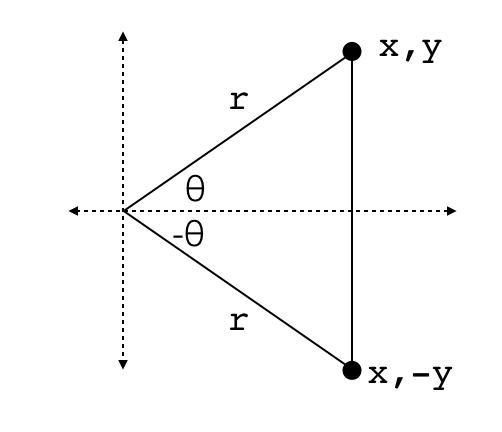
\includegraphics [scale=0.4] {pm_theta.png} \end{center}

The diagram shows the reason:
\[ \cos \theta = x/r = \cos - \theta \]
while
\[ \sin \theta = y/r = -  (\sin - \theta ) = - (-y/r) \]

Substitute $- \sin \theta$ for $\sin - \theta$ and $\cos \theta$ for $\cos - \theta$:
\[ \cos s - t = \cos s \cos - t + \sin s \sin - t \]
\[ = \cos s \cos t - \sin s \sin t \]
and
\[ \sin s - t = \sin s \cos t - \cos s \sin t \]

\subsection*{derivation 2 (Strang)}

For a geometric derivation of the sum of angles formula with minimal setup, I really like this figure from Strang

\begin{center} \includegraphics [scale=0.6] {strang_sum.png} \end{center}

We have the same triangle in the two panels, just rotated clockwise on the right.

The squared distance between two points in the plane is
\[ d^2 = (x_2 - x_1)^2 + (y_2 - y_1)^2 = \Delta x^2 + \Delta y^2 \]
This is just the Pythagorean theorem in disguise.

In the left panel, $t$ is the angle between the lower radius and the $x$-axis, $s$ is the angle between the upper radius and the $x$-axis, and as labeled, $s-t$ is the angle between the two radii.

The distance $d$ squared for the two points on the circle in the left panel is
\[ d^2 = (\cos s - \cos t)^2 + (\sin s - \sin t)^2 \]

Multiply out:
\[ d^2 = \cos^2 s - 2 \cos s \cos t  + \cos^2 t +  \sin^2 s - 2 \sin s \sin t + \sin^2 t \]
We have two copies of $\sin^2 + \cos^2$, one for angle $s$  and one for angle $t$
\[ d^2 = 2 - 2 \cos s \cos t - 2 \sin s \sin t \]

In the right panel, the two radii have been rotated, preserving the same angle between them.
\[  d^2 = (\cos (s-t) - 1)^2 + \sin(s-t)^2 \]
(Don't forget the $1$).
\[ = \cos^2 (s-t) - 2 \cos(s-t) + 1 + \sin^2 (s-t) \]
\[ = 2 - 2 \cos(s-t) \]

Because the included angle hasn't changed, neither has the distance, so we can equate the two expressions.  
\[ 2 - 2 \cos(s-t) = 2 - 2 \cos s \cos t - 2 \sin s \sin t \]
Subtract 2 from both sides, divide by $2$, and change all the signs leaving
\[ \cos (s - t) = \cos s \cos t + \sin s \sin t \]
This is our formula for the cosine of the difference of two angles.

\subsection*{getting to sine}

Strang's derivation gives us the formula for sum and difference of cosines.  To get the formula for the sine in the same way, we would need to mix sine and cosine when computing a distance in his diagram.  I don't know how to do that.

The easiest way to get from cosine to sine is to consider an angle $x$ and its complementary angle $y$, where $x + y = \pi/2$.  We know the cosine and sine are switched for complementary angles

\[ \cos x = \sin y = \sin (\pi/2 - x) \]
\[ \sin x = \cos y = \cos (\pi/2 - x) \]

We have the formula:
\[ \cos s + t = \cos s \cos t - \sin s \sin t \]

Let $u + t = \pi/2$.  Then $\cos u = \sin t$ and $\sin u = \cos t$ so

\[ \cos (s + \pi/2 - u) = \cos s \sin u - \sin s \cos u \]

That's close!  We just need a little manipulation of the left-hand side:
\[ = \cos (\pi/2 - (u - s)) = \sin (u - s) \]

So altogether: 
\[ \sin u - s = \sin u \cos s - \cos u \sin s \]

We can easily change this to the familiar symbols, and obtain the negative by the same considerations as we used above.

Here is an alternative connection which proceeds from the graph of sine and cosine versus the angle.

\begin{center} 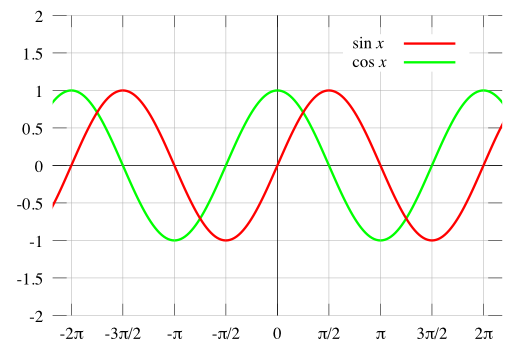
\includegraphics [scale=0.4] {sine_cosine_wikipedia.png} \end{center}

so it's easy to see that $\cos t = \sin t + \pi/2$.

Another approach is to look at the relationships between sine and cosine for angles that are related by addition or subtraction of $\pi/2$.
\begin{center} \includegraphics [scale=0.4] {angles2.png} \end{center}
In the figure, I have simply rotated the same triangle.

\subsection*{sine of the sum}

We compute the area of the triangle in two different ways.  On the left we have that
\[ A = \frac{1}{2} ab \ \sin (\theta + \phi) \]

\begin{center} \includegraphics [scale=0.4] {sum_angles_8.png} \end{center}

On the right, the two smaller triangles are right triangles with $h = a \cos \phi = b \cos \theta$.
\[ A_{top} = \frac{1}{2} a \sin \phi \ b \cos \theta \]
\[ A_{bottom} = \frac{1}{2} b \sin \theta \ a \cos \phi \]
These two expressions add to give the total area.  We can factor out the common $ab/2$ and write the equality:
\[ A = \sin (\theta + \phi) = \sin \phi \cos \theta + \sin \theta \cos \phi \]

\url{https://www.cut-the-knot.org/triangle/SinCosFormula.shtml}

\subsection*{Euler}
Euler's formula is:
\[ e^{i \theta} = \cos \theta + i \sin \theta \]

If you've never seen it before, don't worry what it means or where it comes from.  Just treat $i$ as a constant with $i^2 = -1$.  Multiply as follows:
\[ (\cos s + i \sin s)(\cos t + i \sin t) \]
\[ = \cos s \cos t + i^2 \sin s \sin t + i \ [ \ \sin s \cos t + \cos s \sin t \ ] \] 
\[ = \cos s \cos t - \sin s \sin t + i \ [ \ \sin s \cos t + \cos s \sin t \ ] \] 

This is a \emph{complex} number with a real part (the first two terms), plus an imaginary part, the last two terms, with a leading factor of $i$.

For the same calculation with the exponential
\[ e^{is} \cdot e^{it} = e^{i(s+t)} \]
\[ = \cos (s + t) + i \sin (s + t) \]

By Euler's formula, these two expressions are equal.  

The rule for equality of complex numbers is that both the real parts and the imaginary parts must be equal.  So we have
\[ \cos (s + t) = \cos s \cos t - \sin s \sin t \]
\[ \sin (s + t) = \sin s \cos t + \cos s \sin t \]

\subsection*{vector rotation}

I want to take a moment to introduce a concept that gives another simple proof of the sum of angles theorems.  We don't have time to cover it in the detail it really deserves, that's for later.

Start with the idea of a \emph{vector} from the origin to a point.  Vectors have length --- the vectors depicted are unit vectors with length $1$.  They also have a direction.  The unit vector along the $x$-axis can be represented as the pair of $x,y$-coordinates $(1,0)$.

Let us rotate the vector in the counter-clockwise direction by an angle $\phi$.  The new coordinates of the head of the vector (marked with the arrow) are $(\cos \phi, \sin \phi)$.  We have
\[ 1, 0 \rightarrow \cos \phi, \sin \phi \]
for a vector $x$ units long we have
\[ x, 0 \rightarrow x \cos \phi, x \sin \phi \]
 
By similar reasoning
\[ 0, 1 \rightarrow - \sin \phi, \cos \phi \]
\[ 0, y \rightarrow - y \sin \phi, y \cos \phi \]
We get a minus sign because the rotated unit vector that started pointing straight up is now in the second quadrant, the $x$-component is negative.

\begin{center} \includegraphics [scale=0.4] {rotate_vectors.png} \end{center}

For a general vector $(x,y)$ the resulting vector is $(x',y')$ and the components are:
\[ x' = x \cos \phi - y \sin \phi \]
\[ y' = x \sin \phi + y \cos \phi \]

Now, suppose we rotate a second time, by an angle $\theta$.  Just add a prime for each and substitute $\theta$ for $\phi$.
\[ x'' = x' \cos \theta - y' \sin \theta \]
\[ y'' = x' \sin \theta + y' \cos \theta \]

Write $x''$ in terms of the original $x$ and $y$:
\[ x'' = x' \cos \theta - y' \sin \theta \]
\[ = (x \cos \phi - y \sin \phi) \cos \theta - (x \sin \phi + y \cos \phi) \sin \theta \]
\[ = x \cos \phi \cos \theta - y \sin \phi \cos \theta - x \sin \phi \sin \theta - y \cos \phi \sin \theta \]
\[ = x \ [ \ \cos \phi \cos \theta - \sin \phi \sin \theta \ ] \ - y \ [ \ \sin \phi \cos \theta + \cos \phi \sin \theta \ ] \]

The key idea is that we must get the same result if we turn through both angles at once:
\[ x'' = x ( \cos \phi + \theta) - y (\sin \phi + \theta) \]

The cofactors of $x$ and $y$ must separately be equal:
\[ \cos \phi + \theta = \cos \phi \cos \theta - \sin \phi \sin \theta \]
\[ \sin \phi + \theta = \sin \phi \cos \theta + \cos \phi \sin \theta \]

Those are our formulas!

If you know about matrix multiplication, you can write 

\[ 
\begin{bmatrix}
\ \ \cos s \ \sin s \\
-\sin s \ \cos s 
\end{bmatrix}
\]
and then
\[
\begin{bmatrix}
\ \ \cos s \ \sin s \\
-\sin s \ \cos s 
\end{bmatrix}
\begin{bmatrix}
\ \ \cos t \ \sin t \\
-\sin t \ \cos t 
\end{bmatrix}
= \begin{bmatrix}
\ \ \cos s+t \  \sin s+t \\
- \sin s+t \ \ \cos s+t
\end{bmatrix}
\]
The simple multiplication rule will recover our formulas.

\subsection*{double-angle formulas}
Very quickly, sine:
\[ \sin s + t = \sin s \cos t + \cos s \sin t \]
\[ \sin 2t = 2 \sin t \cos t \]
And cosine:
\[ \cos s + t = \cos s \cos t - \sin s \sin t \]
\[ \cos 2t = \cos^2 t - \sin^2 t = 2 \cos^2 t - 1 \]

Sometimes, it is helpful to have a simpler notation.  If we write $S$ for sine and $C$ for cosine, and use a prime for the double angle:
\[ S' = 2SC \]
\[ C' = 2C^2 - 1 \]
The inverse tangent is
\[ \frac{1}{T'} = \frac{1}{T} - \frac{1}{2SC} = \frac{1}{T} - \frac{1}{S} \]

\subsection*{geometric derivation}

Here is a simple geometric derivation of the double angle formula for sine.

\begin{center} \includegraphics [scale=0.4] {double_angle.png} \end{center}

From our work with arcs, we know that angle $\phi$ on the left is one-half the central angle $\theta$, and from Thales' theorem, that the angle on the circle at the top-right is a right angle.  So the small right triangle with hypotenuse $h$ also has angle $\phi$, as labeled, since they have the same complementary angle.

It helps to know where we're going, as well.  From above:
\[ \sin \theta = 2 \sin \phi \cos \phi \]
\[ \cos \theta = \cos^2 \phi - \sin^2 \phi \]

Because there are two copies of a trig function in each term, we will have a factor of $h^2$ on the bottom:
\[ h^2 = x^2 + y^2 \]
and from the triangle containing $\theta$ we have that
\[ (1-x)^2 + y^2 = 1 \]
\[ x^2 + y^2 = 2x \]

\begin{center} \includegraphics [scale=0.4] {double_angle.png} \end{center}

From the diagram:
\[ 2 \sin \phi \cos \phi = 2 \ \frac{y}{h} \cdot \frac{x}{h} \]
\[ = 2 \ \frac{xy}{2x} \]
\[ = y = \sin \theta \]

$\square$

The same diagram will serve for the cosine.  The double-angle formula is:
\[ \cos \theta = \cos^2 \phi - \sin^2 \phi \]
\[ = \frac{y^2}{h^2} - \frac{x^2}{h^2} \]
\[ = \frac{y^2 - x^2}{2x} \]

But $y^2 = 2x - x^2$:
\[ = \frac{2x -x^2 - x^2}{2x} \]
\[ = 1 - x \]

\begin{center} \includegraphics [scale=0.4] {double_angle.png} \end{center}

$\square$

Similar calculations can be done for a diagram that is slightly relabeled, to provide a simple geometric proof of the Pythagorean theorem.

\begin{center} \includegraphics [scale=0.4] {double_angle_2.png} \end{center}

Thales theorem allows us to deduce that the triangle with two dotted sides is a right triangle, hence the two angles labeled $\phi$ are equal by complementarity with the same angle.  By similar triangles, we have then that
\[ \tan \phi = \frac{y}{r + x} = \frac{r - x}{y} \]
\[ y^2 = r^2 - x^2 \]
\[ x^2 + y^2 = r^2 \]

For the double-angle calculations, there are two triangles with base angle $\phi$ and the hypotenuse a dotted line.  The squared lengths of the two hypotenuses are:
\[ (r + x)^2 + y^2 = r^2 + 2rx + x^2 + y^2 \]
\[ = 2r^2 + 2rx = 2r(r + x) \]
and 
\[ (r - x)^2 + y^2 = r^2 - 2rx + x^2 + y^2 \]
\[ = 2r^2 - 2rx = 2r(r - x) \]

So then the products of $\sin$ and $\cos$ work out to be simple ratios, which in each case will have further cancelations.

As one example, for the large triangle:
\[ \cos^2 \phi - \sin^2 \phi = \frac{(x+r)^2}{2r(r + x)} - \frac{y^2}{2r(r + x)} \]

Let us just work with the numerator for a minute:
\[ (x+r)^2 - y^2 = x^2 + 2xr + r^2 - (r^2 - x^2) \]
\[ 2x^2 + 2xr = 2x(x + r) \]
So we see that $2(x+r)$ cancels and the ratio is just
\[ \frac{x}{r} \]
which is $\cos \theta$.

\subsection*{another calculation}
We found previously that 
\[ \sin \frac{\pi}{4} = \cos \frac{\pi}{4} = \frac{1}{\sqrt{2}} \]
\[ \sin \frac{\pi}{6} = \cos \frac{\pi}{3} = \frac{1}{2} \]
\[ \sin \frac{\pi}{3} = \cos \frac{\pi}{6} = \frac{\sqrt{3}}{2} \]

These angles correspond to 30, 45 and 60 degrees.  It might be nice to have sine and cosine of 15 and 75 degrees as well.  That would make even divisions of the first 90 degrees.  We can get them as the sum and difference of $\pi/4$ and $\pi/6$.

Let $s = \pi/4$ and $t = \pi/6$.  Then

\[ \sin \frac{\pi}{12} = \sin s - t = \sin s \cos t - \sin t \cos s \]
\[ = \frac{1}{\sqrt{2}} \cdot \frac{\sqrt{3}}{2} - \frac{1}{2} \cdot \frac{1}{\sqrt{2}} = \frac{\sqrt{3} - 1}{2 \sqrt{2}} \]
\[ \cos \frac{\pi}{12} = \cos s - t = \cos s \cos t + \sin s \sin t \]
\[ = \frac{\sqrt{3}}{2} \cdot \frac{1}{\sqrt{2}} - \frac{1}{2} \cdot \frac{1}{\sqrt{2}} = \frac{\sqrt{3} + 1}{2 \sqrt{2}} \]

We just check that $\sin^2 \theta + \cos^2 \theta = 1$:
\[ \frac{(\sqrt{3} - 1)^2 + (\sqrt{3} + 1)^2}{(2 \sqrt{2})^2} \]
\[ = \frac{3 - 2 \sqrt{3} + 1 + 3 + 2 \sqrt{3} + 1}{8} = 1 \]

We can calculate similarly for $s + t = 5 \pi/12$ or just switch sine and cosine from $\pi/12$.

\end{document}